\documentclass[xcolor=dvipsnames]{beamer}

% PACKAGES
\usepackage[german,english]{babel}
\usepackage[utf8]{inputenc}
\usepackage{amsmath}
\usepackage{amsfonts}
\usepackage{amssymb}
\usepackage{amsthm}
\usepackage{marvosym}
\usepackage{caption}
\usepackage{diagbox}
\usepackage{tabu}
\usepackage{makecell} % thickhline = \Xhline{2\arrayrulewidth}
\usepackage{tikz}
\usetikzlibrary{arrows,positioning,scopes,automata,calc}

% THEOREM STYLES
\theoremstyle{plain}
\newtheorem{thm}{Theorem}[subsection]
\newtheorem{lem}[theorem]{Lemma}
\newtheorem{prop}[theorem]{Proposition}
\newtheorem*{cor}{Corollary}
\theoremstyle{definition}
\newtheorem{defn}{Definition}[subsection]
\newtheorem{conj}{Conjecture}
\newtheorem{exmp}{Example}[section]
\theoremstyle{remark}
\newtheorem*{rem}{Remark}
\newtheorem*{nte}{Note}
\newtheorem{case}{Case}

% COMMANDS
\newcommand{\enquote}[1]{``#1''}
\newcommand{\regexarrow}{\underset{\raisebox{.4ex}[0pt][0pt]{\small$\uparrow$}}{\,}}

% Redefine \emph
\let\emph\textbf

% SLIDE STYLES
\usetheme{Madrid}
\makeatletter
\setbeamertemplate{footline}
{
  \leavevmode%
  \hbox{%
  \begin{beamercolorbox}[wd=.55\paperwidth,ht=2.25ex,dp=1ex,center]{author in head/foot}%
    \usebeamerfont{author in head/foot}\insertshorttitle
  \end{beamercolorbox}%
  \begin{beamercolorbox}[wd=.35\paperwidth,ht=2.25ex,dp=1ex,center]{title in head/foot}%
    \usebeamerfont{title in head/foot}\insertsection
  \end{beamercolorbox}%
  \begin{beamercolorbox}[wd=.1\paperwidth,ht=2.25ex,dp=1ex,right]{date in head/foot}%
    \insertframenumber{} / \inserttotalframenumber\hspace*{2ex} 
  \end{beamercolorbox}}%
  \vskip0pt%
}
\makeatother

\setbeamertemplate{theorem begin}
{%
\begin{\inserttheoremblockenv}
{%
\inserttheoremheadfont
\inserttheoremname
\inserttheorempunctuation
}%
}
\setbeamertemplate{theorem end}{\end{\inserttheoremblockenv}}
\makeatother

\setbeamertemplate{navigation symbols}{}
\setbeamertemplate{itemize items}[default]
\setbeamertemplate{enumerate items}[default]



% DOCUMET INFORMATION
\title{State Space Reduction For Parity Automata}
\author[Andreas Tollkötter]{Andreas Tollkötter\\{\small Supervisor: Dr. Christof Löding}}
\date{\today}

\begin{document}
{
\setbeamertemplate{footline}{}
\frame{\titlepage}
}

\begin{frame}{Overview}
We establish the notion of \emph{merger functions}. Using that definition, we present three of our newly developed heuristic techniques to reduce the number of states in deterministic parity automata. 

\vspace{.5cm}
\pause

\begin{enumerate}
	\item Deterministic Parity Automata
	\item Why do we need heuristic reduction?
	\item Merger functions as a framework
	\item Delayed Simulation
	\item Congruence Path Refinement
	\item Labeled SCC Filter
\end{enumerate}
\end{frame}

\AtBeginSection[]
{
{
\setbeamertemplate{footline}{}
\setbeamercolor{section in toc}{fg=alerted text.fg}
\setbeamercolor{section in toc shaded}{bg=structure!20,fg=structure}
\setbeamertemplate{section in toc shaded}[default][100]
\begin{frame}<beamer>
  \frametitle{Table Of Contents}
  \tableofcontents[currentsection]
\end{frame}
}
}


\section{Deterministic Parity Automata}
\begin{frame}{$\omega$-automata}
$\omega$-words are words of one-sided infinite length: \\
$\Sigma^\omega = $ functions from $\mathbb{N}$ to $\Sigma$

\vspace{.5cm}

$\omega$-automata are finite transition structures that describe a language $L \subseteq \Sigma^\omega$ 

\vspace{.5cm}

Deterministic parity automata (DPA):
\begin{itemize}
	\item State set $Q$
	\item Alphabet $\Sigma$
	\item Transition function $\delta : Q \times \Sigma \rightarrow Q$
	\item Priority function $c : Q \rightarrow \mathbb{N}$
\end{itemize}

An $\omega$-word $\alpha$ starting in a state $q_0 \in Q$ induces a run $q_0 q_1 q_2 \dots$. \\
The DPA accepts $\alpha$ iff the \emph{smallest} priority that occurs infinitely often in the sequence $c(q_0) c(q_1) c(q_2) \dots$ is \emph{even}.

\end{frame}


\section{Why do we need heuristic reduction?}
\begin{frame}{Why do we need heuristic reduction?}

Goal: Reduce number of states in the automaton to ease run time of follow up algorithms.

\vspace{.7cm}

\textbf{Minimization Problem}: Given an automaton $\mathcal{A}$, what is the smallest number of states required to recognize the same language as $\mathcal{A}$?

\vspace{.7cm}

For DFAs: Minimization is solvable in $\mathcal{O}(n \log n)$. \cite{Hopcroft1971}

For DPAs: Minimization is NP-hard. \cite{Schewe2010}

\end{frame}


\begin{frame}{Moore Minimization}
A DPA can be interpreted as a Moore automaton with $c$ being the output function.

\begin{defn}[Moore equivalence]
	$p \equiv_M q$ iff $\forall w \in \Sigma^*: c(\delta^*(p, w)) = c(\delta^*(q, w))$.
\end{defn}

\vspace{.5cm}
\pause

\begin{theorem}
	Deterministic Moore automata can be minimized in log-linear time.
\end{theorem}

Idea: Build the quotient automaton w.r.t. $\equiv_M$.

\vspace{.5cm}

The same algorithm can be used to reduce DPAs but will not give minimal DPAs in general.
\end{frame}




\section{Merger functions as a framework}
\begin{frame}{Merger functions}
\emph{Merger functions} $\mu$ map from some $D \subseteq 2^Q$ into $2^Q \setminus \{\emptyset\}$.

\vspace{.5cm}

$M, C \subseteq Q$

\begin{equation*}
\tikz[baseline]{\node {$\mu($}} \tikz[baseline]{\node(d4) {$M$}} \tikz[baseline]{\node {$) =$}} \tikz[baseline]{\node(d5){$C$}}
\end{equation*}

\begin{tikzpicture}[remember picture,overlay]
\draw[blue,thick,->] (d4) to [in=90,out=245] + (225:2.7cm) node[anchor=north,text = black] {
	All states from the \emph{merge set} \dots
};
\draw[blue,thick,->] (d5) to [in=90,out=265] +(300:2.8cm) node[anchor=north,text = black] {
	\begin{tabular}{cc}
		\dots can be represented by any single \\
		one representative from the \emph{candidate set}.
	\end{tabular}
};
\end{tikzpicture}

\vfill
\end{frame}

\begin{frame}{Merger functions generalize quotient automata}
Special case: $\mu(M) = M$. \\
Remove all states from $M$ except for one (arbitrarily chosen) representative.

\vspace{.5cm}

For a congruence relation $\sim$, let $\mathfrak{C} \subseteq 2^Q$ be the equivalence classes. \\
The quotient automaton is defined by state set $\mathfrak{C}$. \\
This is captured by the merger function $\mu_\div : \mathfrak{C} \rightarrow 2^Q , \kappa \mapsto \kappa$.
\end{frame}




\section{Delayed Simulation}
\begin{frame}{Delayed Simulation}
\begin{defn}
	$p \equiv_\text{de} q$ iff for all $w \in \Sigma^*$, every run that starts in $\delta^*(p, w)$ or $\delta^*(q, w)$ eventually sees a priority of at most $\min \{c(\delta^*(p, w)), c(\delta^*(q, w))\}$.
\end{defn}
\end{frame}

\begin{frame}{Delayed Simulation}
\begin{figure}
	\centering
	\begin{tikzpicture}[shorten >=1pt,node distance=2cm,on grid,initial text=]
  	\node[state]           (0)                {$p$};
  	\node[state]           (1) [below=of 0]   {$q$};
  	\node           (2) [above right=of 0]   {\dots};
  	\node           (3) [below right=of 1]   {\dots};
  	\node[state]           (4) [below right=of 2]   {$p'$};
  	\node[state]           (5) [above right=of 3]   {$q'$};
  	\node			(6) [below=1cm of 0] {$p \equiv_\text{de} q$};
  	\node			(7) [below=1cm of 4] {$c(p') < c(q')$};
  	\node[state]	(8) [right=4cm of 5] {$q''$};
  	\node	(9) [above=1cm of 8] {$c(q'') \leq c(p')$};
  	\path[-] 	(0) edge [bend left] node [below right] {$w$} (2)
  				(1) edge [bend right] node [above right] {$w$} (3);
  	\path[->]   (2) edge [bend left] node {} (4)
  				(3) edge [bend right] node {} (5);
  	\draw[->,decorate,decoration={snake,amplitude=1mm,segment length=4mm,post length=1mm}] (5) -- node[below] {on all paths} (8);
	\end{tikzpicture}
\end{figure}
\end{frame}

\begin{frame}{Delayed Simulation}
\begin{defn}
	Let $\mathfrak{C}_\text{de} = \{ [q]_{\equiv_\text{de}} \mid q \in Q \}$ be the set of $\equiv_\text{de}$-equivalence classes. \\
	Define the \emph{delayed simulation merger} as $$\mu_\text{de} : \mathfrak{C}_\text{de} \rightarrow 2^Q, \kappa \mapsto \{ q \in \kappa \mid c(q) = \min c(\kappa) \}.$$
\end{defn}

\begin{theorem}
	Merging states according to $\mu_\text{de}$ preserves language.
\end{theorem}
\end{frame}


\begin{frame}{Computing Delayed Simulation}
	We define a det.\ Büchi automaton $\mathcal{G}_\text{de}$ with states $q_\text{de}^0(p, q)$ such that: \\
	$p \equiv_\text{de} q$ iff both $L(\mathcal{G}_\text{de}, q_\text{de}^0(p, q))$ and $L(\mathcal{G}_\text{de}, q_\text{de}^0(q, p))$ are universal ($\Sigma^\omega$).
	
	\vspace{.5cm}
	
	This automaton uses the state set $Q_\text{de} = Q \times Q \times (c(Q) \cup \{\checkmark\})$. \\
	Computing states of universal language in a DBA requires linear time.
	
	\vspace{.5cm}
	
	\begin{theorem}
		$\mu_\text{de}$ can be computed in $\mathcal{O}(n^2 k)$.
	\end{theorem}
\end{frame}

\begin{frame}{Delayed Simulation Automaton}
$\mathcal{G}_\text{de} = (Q_\text{de}, \Sigma, \delta_\text{de}, F_\text{de})$

\begin{itemize}
	\item States are $Q_\text{de} = Q \times Q \times (c(Q) \cup \{\checkmark\})$. \\
The first two components are a \enquote{simulation} of the original DPA. The third component are the so called \enquote{obligations}.
	\item Transitions $\delta_\text{de}$.
\begin{align*}
	\delta_\text{de}((p, q, k), a) = (& \delta(p, a), \\
									& \delta(q, a), \\
									& \gamma( \quad c(\delta(p, a)), \quad c(\delta(q, a)), \quad k \quad ))
\end{align*}
	\item Accepting states are $F_\text{de} = Q \times Q \times \{\checkmark\}$.
\end{itemize}

\end{frame}


\begin{frame}{Delayed Simulation Automaton: $\gamma$}
	(Actual definition of $\gamma$ is more complex for some additional properties.) \\
	
	\vspace{.5cm}
	
	$\gamma : \mathbb{N} \times \mathbb{N} \times (\mathbb{N} \cup \{\checkmark\}) \rightarrow \mathbb{N} \cup \{\checkmark\}$
	
	\begin{align*}
		& \gamma(i, j, \checkmark) = \begin{cases}
			\checkmark & \text{if } j \leq i \\
			i & \text{else}
		\end{cases} \\
		\text{for } k \in \mathbb{N}: \quad & \gamma(i, j, k) = \begin{cases}
			\checkmark & \text{if } j \leq \min \{i, k\} \\
			\min \{i, k\} & \text{else}
		\end{cases}
	\end{align*}
	
	\vspace{.5cm}
	
	$q_\text{de}^0(p, q) = (p, q, \gamma(c(p), c(q), \checkmark))$.
\end{frame}


\begin{frame}{Delayed Simulation Automaton: $\gamma$}
	Let $0 \leq_\checkmark 1 \leq_\checkmark 2 \leq_\checkmark \dots \leq_\checkmark \checkmark$.

	For $p, q \in Q$, $k \in c(Q) \cup \{\checkmark\}$, $a \in \Sigma$, set $\gamma((p, q, k), a) = \gamma'(\delta^*(p, a), \delta^*(q, a), k)$, where $\gamma'$ is defined as follows: \\
	If any of the following is true, then $\gamma'(i, j, k) = \checkmark$.
	
	\begin{itemize}
		\item $i$ is odd, $j$ is even, and $i \leq_\checkmark k$
		\item $i$ is odd, $j$ is even, and $j \leq_\checkmark k$
		\item $i$ is odd, $j$ is odd, $j \geq i$, and $i \leq_\checkmark k$
		\item $i$ is even, $j$ is even, $j \leq i$, and $j \leq_\checkmark k$
	\end{itemize}
	
	Otherwise, $\gamma'(i, j, k) = min_{\leq_\checkmark} \{ i,j,k \}$.
	
	$q_\text{de}^0(p, q) = (p, q, \gamma'(c(p), c(q), \checkmark))$.
\end{frame}


\begin{frame}{Delayed Simulation Automaton}
\begin{figure}
\centering
\begin{tikzpicture}[shorten >=1pt,node distance=2cm,on grid,initial text=]
  \node[state]           (0)                {$q_0,1$};
  \node[state]           (1) [right=of 0]   {$q_1,1$};
  \node[state]           (2) [above=of 0]   {$q_2,1$};
  \node[state]           (3) [right=of 2]   {$q_3,1$};
  \node[state]           (4) [right=of 3]   {$q_4,0$};
  \path[->] (0) edge [bend left] node [above] {a} (1)
  			(0) edge node [left] {b} (2)
            (1) edge [bend left] node [below] {a} (0)
            (1) edge node [below] {b} (4)
            (2) edge [bend left] node [above] {a,b} (3)
            (3) edge [bend left] node [below] {a} (2)
            (3) edge [bend left] node [above] {b} (4)
            (4) edge [bend left] node [below] {a,b} (3);
\end{tikzpicture}
\end{figure}

A DPA with 5 states. We want to check whether $q_0 \equiv_\text{de} q_1$ is true. 
\end{frame}

\begin{frame}{Delayed Simulation Automaton}
\begin{figure}
\centering
\begin{tikzpicture}[shorten >=1pt,node distance=2.9cm,on grid,initial text=]
  \node[state,accepting,onslide=<2>{highlight}] (0)			    {$q_0,q_1,\checkmark$};
  \node[state,accepting] (1) [right=of 0]   {$q_2,q_4,\checkmark$};
  \node[state,accepting] (2) [right=of 1]   {$q_3,q_3,\checkmark$};
  \node[state,accepting,onslide=<3>{highlight}] (3) [below=of 0]   {$q_1,q_0,\checkmark$};
  \node[state,onslide=<4>{highlight}] 			 (4) [right=of 3]   {$q_4,q_2,0$};
  \node[state,onslide=<5>{highlight},onslide=<7>{highlight}] 			 (5) [right=of 4]   {$q_3,q_3,0$};
  \node[state,accepting] (6) [right=of 5]   {$q_4,q_4,\checkmark$};
  \node[state,onslide=<6-7>{highlight}] 			 (7) [below=of 5]   {$q_2,q_2,0$};
  \node[state,accepting] (8) [right=of 2]   {$q_2,q_2,\checkmark$};
  \path[->] (0) edge node [above] {a} (1)
  			(0) edge [bend left] node [right] {b} (3)
            (1) edge node [above] {a,b} (2)
            (2) edge node [above] {a} (6)
            (2) edge [bend left] node [above] {b} (8)
            (3) edge node [above] {a} (4)
            (3) edge [bend left] node [left] {b} (0)
            (4) edge node [above] {a,b} (5)
            (5) edge [bend left,onslide=<7>{highlight}] node [right] {a} (7)
            (5) edge node [above] {b} (6)
            (6) edge [bend left] node [right] {a,b} (2)
            (7) edge [bend left,onslide=<7>{highlight}] node [left] {a,b} (5)
            (8) edge node [above] {a,b} (2);
\end{tikzpicture}
\end{figure}
\end{frame}


\begin{frame}{Efficiency}
\begin{figure}
	\centering
	\includegraphics[page=6,height=.8\textheight]{../data/analysis/fritzwilke/detnbaut_ap1.pdf} 
\end{figure}
\end{frame}




\section{Congruence Path Refinement}
\begin{frame}{Congruence Path Refinement}
	\begin{defn}
	Let $\sim$ be a congruence relation and let $\lambda \subseteq Q$ be an equivalence class of $\sim$. \\
	We define $L_{\lambda \hookleftarrow} \subseteq \Sigma^*$ as the set of all words such that the induced run from a state in $\lambda$ moves back to $\lambda$ exactly once and ends there. \\ 
	The \emph{path refinement} equivalence $\equiv_\text{PR}^\lambda$ is the largest relation such that if $p \equiv_\text{PR}^\lambda q$, then for all $w \in L_{\lambda \hookleftarrow}$, $\delta^*(p, w) \equiv_\text{PR}^\lambda \delta^*(q, w)$ and the smallest priority seen when reading $w$ is the same from $p$ and from $q$.
	\end{defn}
\end{frame}



\begin{frame}{Path Refinement Relation}
\begin{figure}
\centering
\begin{tikzpicture}[shorten >=1pt,node distance=2cm,on grid,initial text=]
  \node[state]           (0)                {$q_0,1$};
  \node[state]           (1) [right=of 0]   {$q_1,1$};
  \node[state]           (2) [above=of 0]   {$q_2,1$};
  \node[state]           (3) [right=of 2]   {$q_3,1$};
  \node[state]           (4) [right=of 3]   {$q_4,0$};
  \path[->] (0) edge [bend left] node [above] {a} (1)
  			(0) edge node [left] {b} (2)
            (1) edge [bend left] node [below] {a} (0)
            (1) edge node [below] {b} (4)
            (2) edge [bend left] node [above] {a,b} (3)
            (3) edge [bend left] node [below] {a} (2)
            (3) edge [bend left] node [above] {b} (4)
            (4) edge [bend left] node [below] {a,b} (3);
\end{tikzpicture}
\end{figure}

Potential choices for $\lambda$ are the equivalence classes of $\equiv_L$: \\ 
$\{q_0, q_1\}$, $\{q_2, q_4\}$, or $\{q_3\}$.
\end{frame}



\begin{frame}{Path Refinement Merger}
\begin{defn}
	Let $\mathfrak{C}_\text{PR}^\lambda = \{ [q]_{\equiv_\text{PR}^\lambda} \mid q \in Q \}$ be the set of $\equiv_\text{PR}^\lambda$-equivalence classes. Define the \emph{path refinement merger} as $\mu_\text{PR}^\lambda : \mathfrak{C}_\text{PR}^\lambda \rightarrow 2^Q, \kappa \mapsto \{ q \in \kappa \mid c(q) = \min c(\kappa) \}$.
\end{defn}

\begin{theorem}
	If all states in $\lambda$ are pairwise language equivalent, merging states according to $\mu_\text{PR}^\lambda$ preserves language.
\end{theorem}
\end{frame}


\begin{frame}{Computing Path Refinement}
	\begin{defn}
		Define the \emph{visit graph} DPA $\mathcal{A}_\text{visit}^\lambda = (Q_\text{visit}^\lambda, \Sigma, \delta_\text{visit}^\lambda, c_\text{visit}^\lambda)$.
		\begin{itemize}
			\item $Q_\text{visit}^\lambda = ((Q \setminus \lambda) \times c(Q) \times \{-1\}) \;\cup\; (\lambda \times c(Q) \times c(Q))$.
			\item $\delta^\lambda_\text{visit}((q, k, k'), a) = \begin{cases}
				(q', \min \{k, c(q')\}, -1) & \text{if } q' \notin \lambda \\
				(q', c(q'), \min \{k, c(q')\}) & \text{if } q' \in \lambda
			\end{cases}$, where $q' = \delta(q, a)$.
			\item $c_\text{visit}^\lambda((q, k, k')) = k'$.
		\end{itemize}
	\end{defn}
	
	States consist of three components $q \in Q \times c(Q) \times (c(Q) \cup \{-1\})$. \\
	The first component \enquote{simulates} the original automaton $\mathcal{A}$. \\
	The second component tracks the minimal priority seen on one run from $\lambda$ to $\lambda$. \\
	The third component is required to distinguish the different priorities.
\end{frame}


\begin{frame}{Computing Path Refinement}
	Moore equivalence in $\mathcal{A}_\text{visit}^\lambda$ corresponds to path refinement equivalence in $\mathcal{A}$.
	
	\begin{theorem}
		$p \equiv_\text{PR}^\lambda q$ iff $(p, c(p), \max c(Q)) \equiv_M (q, c(q), \max c(Q))$.
	\end{theorem}
	
	\begin{theorem}
		$\equiv_\text{PR}^\lambda$ can be computed in $\mathcal{O}(k^2 n \log n)$.
	\end{theorem}
\end{frame}


\begin{frame}{Visit Graph}
\begin{figure}
\centering
\begin{tikzpicture}[shorten >=1pt,node distance=2cm,on grid,initial text=]
  \node[state]           (0)                {$q_0,1$};
  \node[state]           (1) [right=of 0]   {$q_1,1$};
  \node[state]           (2) [above=of 0]   {$q_2,1$};
  \node[state]           (3) [right=of 2]   {$q_3,1$};
  \node[state]           (4) [right=of 3]   {$q_4,0$};
  \path[->] (0) edge [bend left] node [above] {a} (1)
  			(0) edge node [left] {b} (2)
            (1) edge [bend left] node [below] {a} (0)
            (1) edge node [below] {b} (4)
            (2) edge [bend left] node [above] {a,b} (3)
            (3) edge [bend left] node [below] {a} (2)
            (3) edge [bend left] node [above] {b} (4)
            (4) edge [bend left] node [below] {a,b} (3);
\end{tikzpicture}
\end{figure}

Potential choices for $\lambda$ are the equivalence classes of $\equiv_L$: \\ 
$\{q_0, q_1\}$, $\{q_2, q_4\}$, or $\{q_3\}$.
\end{frame}

\begin{frame}{Visit Graph}

$\mathcal{A}_\text{visit}^{\{q_2, q_4\}}$

\begin{figure}
\centering
\begin{tikzpicture}[shorten >=1pt,node distance=2.5cm,on grid,initial text=]
  \node[state]           (0)                {$q_2,1,0$};
  \node[state]           (1) [right=of 0]   {$q_3,0,-1$};
  \node[state]           (2) [below=of 0]   {$q_3,1,-1$};
  \node[state]           (3) [right=of 2]   {$q_4,0,0$};
  \node[state]           (4) [left=of 2]   {$q_2,1,1$};
  \node[state]           (5) [right=of 1]   {$q_4,0,1$};
  \path[->] (0) edge node [left] {a,b} (2)
  			(1) edge node [above] {a} (0)
  			(1) edge [bend left] node [right] {b} (3)
  			(2) edge [bend left] node [above] {a} (4)
  			(2) edge node [above] {b} (3)
  			(3) edge [bend left] node [left] {a,b} (1)
  			(4) edge [bend left] node [above] {a,b} (2)
  			(5) edge node [above] {a,b} (1);
\end{tikzpicture}
\end{figure}
\end{frame}

\begin{frame}{Efficiency}
\begin{figure}
	\centering
	\includegraphics[page=6,height=.8\textheight]{../data/analysis/path_refinement/detnbaut_ap1.pdf} 
\end{figure}
\end{frame}





\section{Labeled SCC Filter}

\begin{frame}{Labeled SCC Filter}
\begin{defn}
	Define $\equiv_M^{\leq k}$ as the Moore equivalence that considers all priorities \emph{greater than k} to be equal. \\
	$p \equiv_M^{\leq k} q$ iff for all $w \in \Sigma^*$: $c(\delta^*(p, w)) = c(\delta^*(q, w))$ or $k < c(\delta^*(p, w)), c(\delta^*(q, w))$.
\end{defn}

\begin{defn}
	Let $\sim$ be an equivalence relation and $k \in \mathbb{N}$. We define the LSF relation $p \equiv^{k,\sim}_\text{LSF} q$ iff $p \sim q$ and $p \equiv_M^{\leq k} q$.
\end{defn}
\end{frame}


\begin{frame}{LSF Relation}
\begin{figure}
\centering
\begin{tikzpicture}[shorten >=1pt,node distance=2cm,on grid,initial text=]
  \node[state]           (0)                {$q_0,0$};
  \node[state]           (1) [below left=of 0]   {$q_1,2$};
  \node[state]           (2) [below right=of 0]   {$q_3,4$};
  \node[state]           (3) [below=of 1]   {$q_2,3$};
  \node[state]           (4) [below=of 2]   {$q_4,5$};
  \path[->] (0) edge [bend left] node [below] {a} (2)
  			(0) edge [bend left] node [above] {b} (1)
  			(1) edge [bend left] node [above] {a} (0)
  			(1) edge [bend left] node [right] {b} (3)
  			(2) edge [bend left] node [below] {a} (0)
  			(2) edge [bend left] node [right] {b} (4)
  			(3) edge [bend left] node [left] {a} (1)
  			(3) edge [loop left] node [left] {b} (3)
  			(4) edge [bend left] node [left] {a} (2)
  			(4) edge [loop right] node [right] {b} (4);
\end{tikzpicture}
\end{figure}

Equivalence classes of $\equiv_\text{LSF}^{1,\equiv_L}$: $\{q_0\}$, $\{q_1, q_3\}$, and $\{q_2, q_4\}$.
\end{frame}


\begin{frame}{LSF Merger}
From the DPA $\mathcal{A}$, we remove all states which have priority less or equal to $k$ and call the resulting (possibly incomplete) DPA $\mathcal{A}_k$. \\
We choose some total preorder $\preceq_k$ on the states of $\mathcal{A}_k$ such that $p$ being reachable from $q$ in $\mathcal{A}_k$ implies $q \preceq_k p$, and $p \preceq_k q \preceq_k p$ is only true if $p$ and $q$ are in the same SCC in $\mathcal{A}_k$. ($\preceq_k$ is a total preorder that is a minimal extension of reachability.)

\vspace{1cm}

In focus are the set of states that are $\preceq_k$-maximal among a given set $P \subseteq Q$. These are all states in one SCC of $\mathcal{A}_k$ such that no other states in $P$ are reachable.
\end{frame}


\begin{frame}{LSF Merger}
\begin{defn}
	Let $\mathfrak{C}_\text{LSF}^{k,\sim}$ be the set of equivalence classes in $\equiv_\text{LSF}^{k,\sim}$ and let $\kappa$ be such an equivalence class. Define
	$$C_\kappa^k = \{ r \in \kappa \mid c(r) > k \text{ and } r \text{ is } \preceq_k \text{-maximal among } \kappa \}$$
	and $M_\kappa^k = \kappa \setminus C_\kappa^k$.
\end{defn}

\begin{defn}
	Define the \emph{LSF merger function} $$\mu_\text{LSF}^{k,\sim} : \{ M_\kappa^k \mid \kappa \in \mathfrak{C}_\text{LSF}^{k,\sim} \} \rightarrow 2^Q , M_\kappa^k \mapsto C_\kappa^k$$
\end{defn}

\begin{theorem}
	If $\sim$ implies language equivalence, merging states according to $\mu_\text{LSF}^{k,\sim}$ preserves language.
\end{theorem}
\end{frame}


\begin{frame}{LSF example}
\begin{figure}
\centering
\begin{tikzpicture}[shorten >=1pt,node distance=2cm,on grid,initial text=]
  \node[state]           (0)                {$q_0,0$};
  \node[state]           (1) [below left=of 0]   {$q_1,2$};
  \node[state]           (2) [below right=of 0]   {$q_3,4$};
  \node[state]           (3) [below=of 1]   {$q_2,3$};
  \node[state]           (4) [below=of 2]   {$q_4,5$};
  \path[->] (0) edge [bend left] node [below] {a} (2)
  			(0) edge [bend left] node [above] {b} (1)
  			(1) edge [bend left] node [above] {a} (0)
  			(1) edge [bend left] node [right] {b} (3)
  			(2) edge [bend left] node [below] {a} (0)
  			(2) edge [bend left] node [right] {b} (4)
  			(3) edge [bend left] node [left] {a} (1)
  			(3) edge [loop left] node [left] {b} (3)
  			(4) edge [bend left] node [left] {a} (2)
  			(4) edge [loop right] node [right] {b} (4);
\end{tikzpicture}
\end{figure}

Equivalence classes of $\equiv_\text{LSF}^{1,\equiv_L}$: $\{q_0\}$, $\{q_1, q_3\}$, and $\{q_2, q_4\}$.
\end{frame}


\begin{frame}{LSF example}
$\mathcal{A}_1$ variant of the automaton.

\begin{figure}
\centering
\begin{tikzpicture}[shorten >=1pt,node distance=2cm,on grid,initial text=]
  \node           (0)                {};
  \node[state]           (1) [below left=of 0]   {$q_1,2$};
  \node[state]           (2) [below right=of 0]   {$q_3,4$};
  \node[state]           (3) [below=of 1]   {$q_2,3$};
  \node[state]           (4) [below=of 2]   {$q_4,5$};
  \path[->] (1) edge [bend left] node [right] {b} (3)
  			(2) edge [bend left] node [right] {b} (4)
  			(3) edge [bend left] node [left] {a} (1)
  			(3) edge [loop left] node [left] {b} (3)
  			(4) edge [bend left] node [left] {a} (2)
  			(4) edge [loop right] node [right] {b} (4);
\end{tikzpicture}
\end{figure}

Possible order: $q_1 \simeq_1 q_2 \prec_1 q_3 \simeq_1 q_4$. \\
$q_3$ is the only $\preceq_1$-maximal element in $\{q_1, q_3\}$. \\
$q_4$ is the only $\preceq_1$-maximal element in $\{q_2, q_4\}$.

$\mu_\text{LSF}^{1,\equiv_L}(\{q_1\}) = \{q_3\}$ \\
$\mu_\text{LSF}^{1,\equiv_L}(\{q_2\}) = \{q_4\}$
\end{frame}


\begin{frame}{LSF example}
After the merge:

\begin{figure}
\centering
\begin{tikzpicture}[shorten >=1pt,node distance=2cm,on grid,initial text=]
  \node[state]           (0)                {$q_0,0$};
  \node[state]           (2) [below=of 0]   {$q_3,4$};
  \node[state]           (4) [below=of 2]   {$q_4,5$};
  \path[->] (0) edge [bend left] node [right] {a,b} (2)
  			(2) edge [bend left] node [left] {a} (0)
  			(2) edge [bend left] node [right] {b} (4)
  			(4) edge [bend left] node [left] {a} (2)
  			(4) edge [loop right] node [right] {b} (4);
\end{tikzpicture}
\end{figure}
\end{frame}



\begin{frame}{Computing LSF}
	The definition provides a straight-forward computation: $\equiv_M^{\leq k}$ is only a slight variation of the normal Moore equivalence and $\preceq_k$ can be computed with a topological sorting on the SCCs of $\mathcal{A}_k$.
	
	\begin{theorem}
		$\mu_\text{LSF}^{k,\sim}$ can be computed in $\mathcal{O}(n \log n)$.
	\end{theorem}
\end{frame}



\begin{frame}{Efficiency}
\begin{figure}
	\centering
	\includegraphics[page=6,height=.8\textheight]{../data/analysis/lsf/detnbaut_ap1.pdf} 
\end{figure}
\end{frame}


















\begin{frame}[allowframebreaks]
\nocite{*}
\bibliographystyle{plain}
\bibliography{citations}
\end{frame}
\end{document}
